\documentclass{article}

\usepackage{graphicx}
\usepackage{tikz}
\usepackage{tikzsymbols}
\usetikzlibrary{calc,patterns,shapes.geometric}
\pagestyle{empty}
\usepackage[margin=0pt]{geometry}
\geometry{papersize={14in,12in}}

\def\centerarc[#1](#2)(#3:#4:#5){\draw[#1] ($(#2)+({#5*cos(#3)},{#5*sin(#3)})$) arc (#3:#4:#5);}

\begin{document}
	\begin{figure}
		\centering
		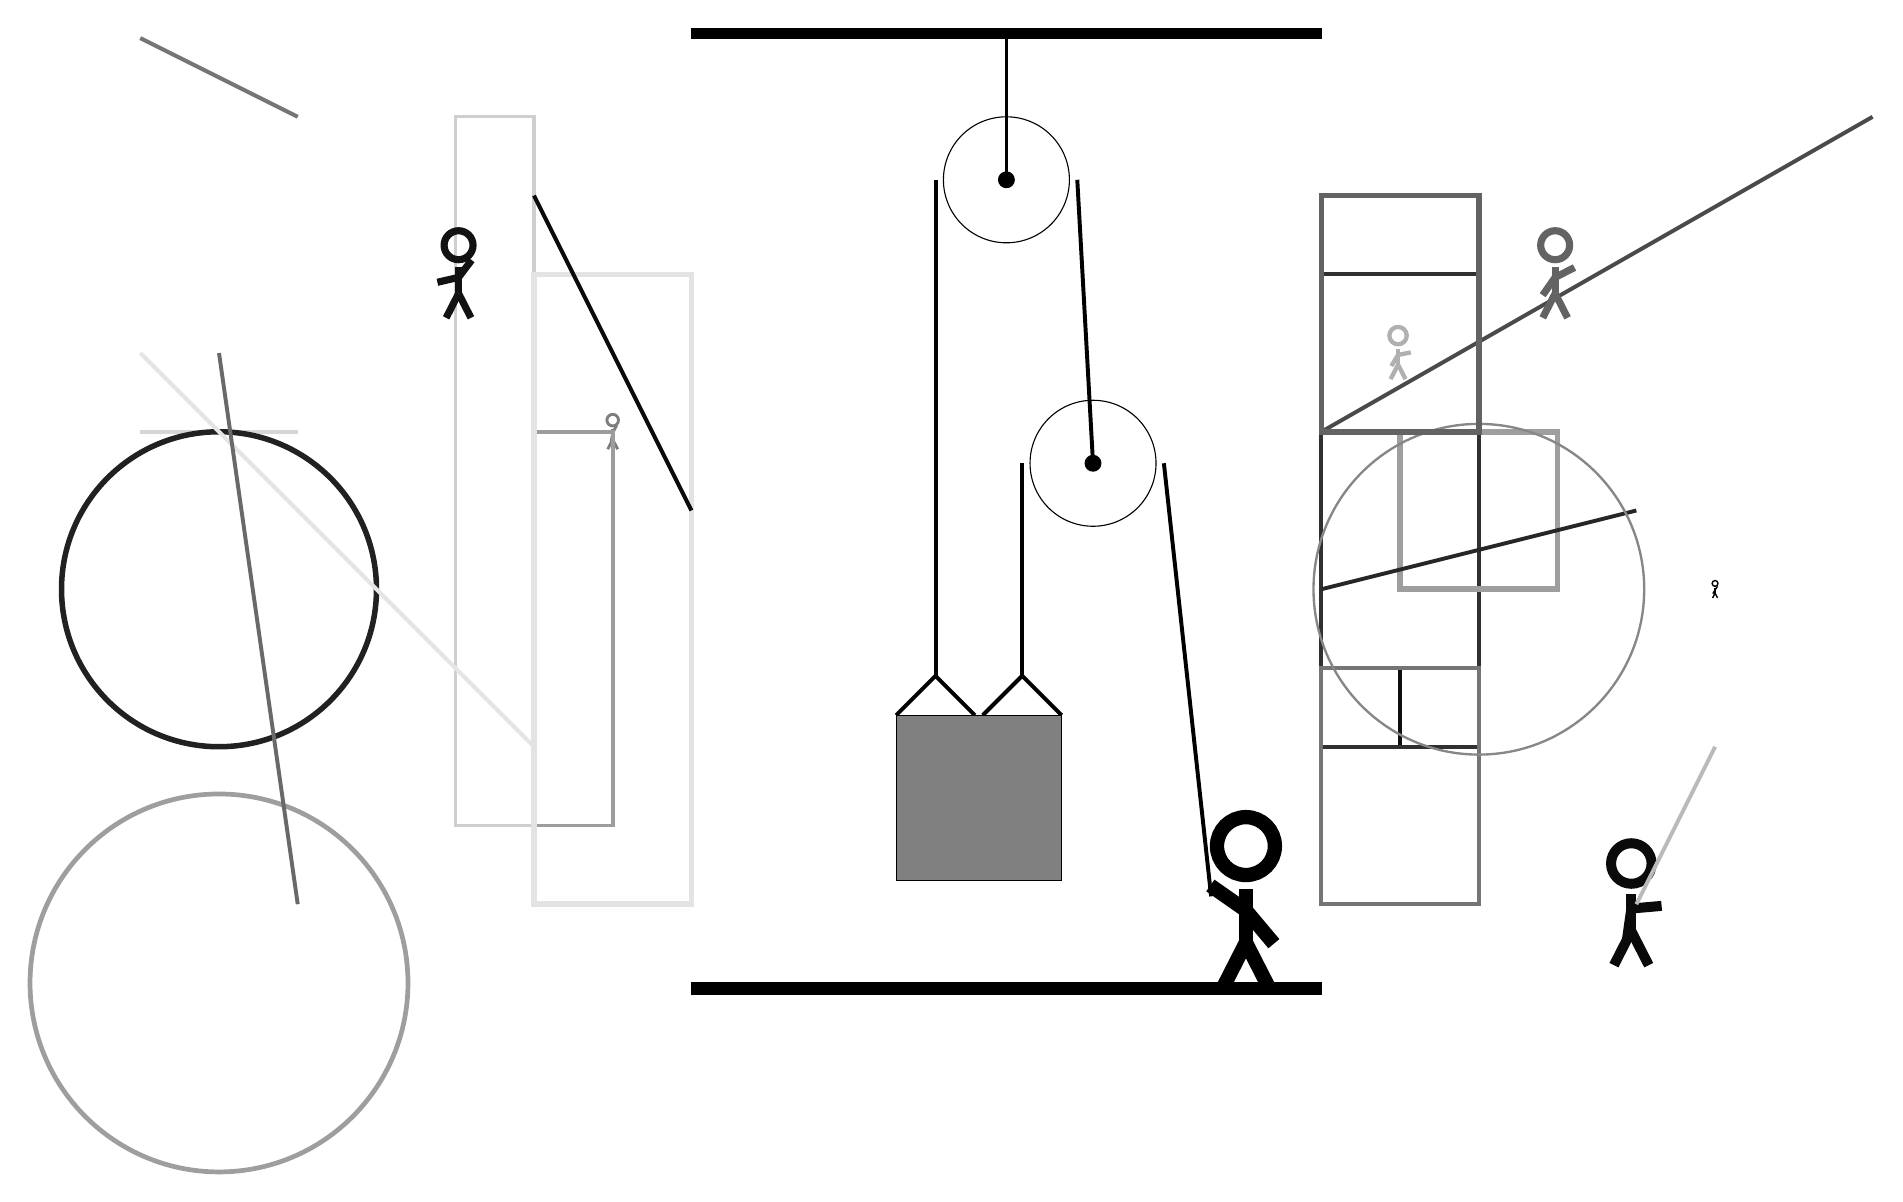
\begin{tikzpicture}
			%%%%% START %%%%%
			
			\draw[fill=black] (-2, 9) rectangle (6, 9.125);
			
			\draw (2, 7.2) circle (0.8);
			\draw[fill=black] (2, 7.2) circle (0.1);
			\draw[thick] (2, 7.2) -- (2, 9);
			
			\draw (3.1, 3.6) circle (0.8);
			\draw[fill=black] (3.1, 3.6) circle (0.1);
			
			\draw[line width = 0.5mm]  (0.6, 0.4) -- (1.1, 0.9) -- (1.6, 0.4);
			\draw[line width = 0.5mm]  (1.7, 0.4) -- (2.2, 0.9) -- (2.7, 0.4);
			\draw[fill=black!50] (0.6, 0.4) rectangle (2.7, -1.7);
			
			\draw[line width = 0.5mm] (1.1, 7.2) -- (1.1, 0.9);
			\centerarc[line width = 0.5mm](2, 7.2)(0:180:0.9);
			\draw[line width = 0.5mm] (2.9, 7.2) -- (3.1, 3.6);
			\draw[line width = 0.5mm] (2.2, 3.6) -- (2.2, 0.9);
			\centerarc[line width = 0.5mm](3.1, 3.6)(0:180:0.9);
			\draw[line width = 0.5mm] (4.0, 3.6) -- (4.6, -1.9);
			
			\node at (5, -2) {\Strichmaxerl[10][-35][-50]};
			
			\draw[line width=0.5mm, color=black!54](-7, 8) -- (-9, 9);
			
			\draw[line width=0.5mm, color=black!71](6, 4) -- (13, 8);
			\draw[line width=0.5mm, color=black!94] (7, 1) rectangle (7, 0);
			\draw [line width=0.3mm, color=black!30](10, -2) circle (0.0);
			\draw[line width=0.5mm, color=black!81] (6, 6) rectangle (8, 0);
			
			\draw[line width=0.5mm, color=black!16](-7, 4) -- (-9, 4);
			
			\draw[line width=0.5mm, color=black!54] (8, -2) rectangle (6, 1);
			\node[line width=0.3mm, color=black!96] at (10, -2) {\Strichmaxerl[7][82][5]};
			\node[line width=0.5mm, color=black!61] at (9, 6) {\Strichmaxerl[5][55][27]};
			
			\draw [line width=0.6mm, color=black!38](-8, -3) circle (2.4);
			\draw[line width=0.7mm, color=black!38] (7, 4) rectangle (9, 2);
			\draw[line width=0.5mm, color=black!85](6, 2) -- (10, 3);
			\draw [line width=0.7mm, color=black!87](-8, 2) circle (2.0);
			\draw[line width=0.4mm, color=black!19] (-4, 8) rectangle (-5, -1);
			\draw[line width=0.5mm, color=black!27](11, 0) -- (10, -2);
			\draw [line width=0.3mm, color=black!47](8, 2) circle (2.1);
			
			\node[line width=0.6mm, color=black!31] at (7, 5) {\Strichmaxerl[3][59][11]};
			\draw[line width=0.7mm, color=black!61] (8, 4) rectangle (6, 7);
			\node[line width=0.6mm, color=black!51] at (-3, 4) {\Strichmaxerl[2][80][63]};
			
			\node[line width=0.6mm, color=black!99] at (11, 2) {\Strichmaxerl[1][59][54]};
			\draw[line width=0.5mm, color=black!39] (-3, 4) rectangle (-4, -1);
			\node[line width=0.2mm, color=black!93] at (-5, 6) {\Strichmaxerl[5][13][53]};
			
			\draw[line width=0.2mm, color=black!14] (-3, 5) rectangle (-3, 5);
			\draw[line width=0.5mm, color=black!10](-4, 0) -- (-9, 5);
			\draw[line width=0.7mm, color=black!11] (-4, -2) rectangle (-2, 6);
			
			\draw[line width=0.5mm, color=black!59](-7, -2) -- (-8, 5);
			
			\draw[line width=0.5mm, color=black!96](-2, 3) -- (-4, 7);
			
			\draw[fill=black] (-2, -3) rectangle (6, -3.15);
			
			%%%%% END %%%%%
		\end{tikzpicture}
	\end{figure}	
\end{document}